\documentclass[12pt, letter]{article}
\usepackage{xcolor}
\usepackage{./Estilos/ColoresLatex}
\usepackage[utf8]{inputenc}
\usepackage[T1]{fontenc}
\usepackage[spanish]{babel}
\usepackage{amsmath}
\usepackage{amsthm}
\usepackage{physics}
\usepackage{tikz}
\usepackage{float}
\usepackage{siunitx}
\usepackage{multicol}
\usepackage[left=2.00cm, right=2.00cm, top=2.00cm, 
     bottom=2.00cm]{geometry}
\usepackage{pdfpages}

% \renewcommand{\questionlabel}{\thequestion}
\newcommand{\textocolor}[2]{\textbf{\textcolor{#1}{#2}}}
\decimalpoint

\setlength{\belowdisplayskip}{-0.5pt}

\usepackage{tasks}
\settasks{
    label=\Alph*), 
    label-align=left,
    item-indent={20pt}, 
    column-sep={4pt},
    label-width={16pt},
}

\sisetup{per-mode=symbol}

\title{Guía para el examen ordinario - Física IV (Área II)}
\date{}

\begin{document}

\maketitle

\section{Las ondas.}

\subsection{Las ondas en física.}


\begin{figure}[H]
    \centering
    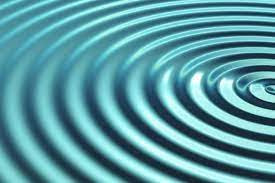
\includegraphics[scale=0.9]{Imagenes/Ondas_01.jpg}
\end{figure}
\begin{figure}[H]
    \centering
    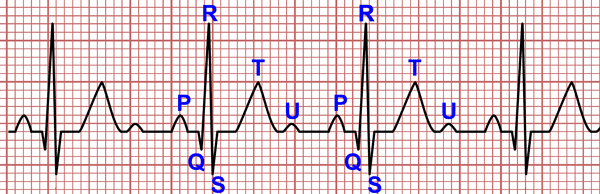
\includegraphics[scale=0.5]{Imagenes/Ondas_02.png}
\end{figure}
\begin{figure}[H]
    \centering
    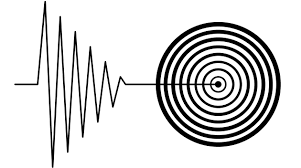
\includegraphics[scale=0.6]{Imagenes/Ondas_03.png}
\end{figure}


\section{El sonido.}

\subsection{El sonido es una onda.}


\textbf{¿Cómo explicamos el sonido?}

De manera inicial debemos de considerar que la definición física del sonido es un concepto, y otro distinto es la sensación fisiológica del mismo.

El sonido es un alteración mecánica que provoca un movimiento ondulatorio a través de medios elásticos (sólidos, líquidos o gaseosos) en todas las direcciones, en forma de ondas longitudinales de presión sonora.
\par
Este fenómeno físico tiene su origen en las vibraciones mecánicas de la materia, generalmente un sólido que transmite la vibración a las partículas contiguas de aire, u otro medio de propagación, en contacto con el mismo, pero sin arrastrarlas. Produciendo de forma alternativa depresiones y sobrepresiones que se van transmitiendo a las capas de aire adyacentes.

\begin{figure}[H]
\centering
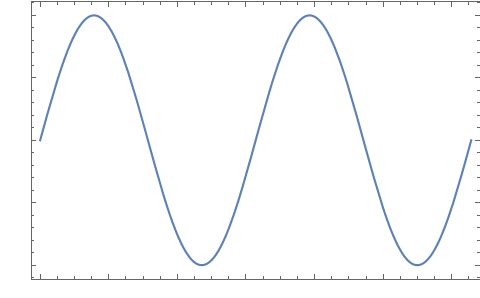
\includegraphics[scale=0.7]{Imagenes/Plot_Onda_01.png}
\end{figure}

Dando lugar a una onda de presión que se propaga con movimiento ondulatorio en todas las direcciones y alejándose del foco. 

\begin{figure}[H]
\centering
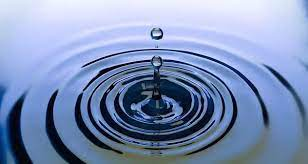
\includegraphics[scale=0.7]{Imagenes/Ondas_04.png}
\end{figure}

Cuando el sonido se transmite, hay un transporte de energía sin transporte de materia.

\subsection{Sonido como sensación.}

El oído transforma las presiones acústicas en sensación auditiva. Que es aquella engendrada en nuestro oído por una onda acústica y por la tanto siempre con un sentido subjetivo ya que depende del receptor de ésta.

\begin{figure}[H]
\centering
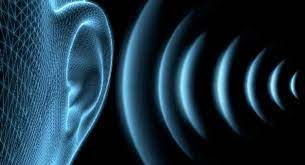
\includegraphics[scale=0.7]{Imagenes/Ondas_05.jpg}
\end{figure}

Las variaciones de presión generadas por las ondas sonoras provocan la vibración del tímpano, situado en el oído, transmitiéndose a una cadena de huesecillos, lo que hace que por medio una serie de mecanismos la sensación sonora llegue al cerebro mediante el nervio auditivo.

% El sonido en sí es de cierta forma una onda. En cualquier disturbio vibratorio que, propagado a través de un medio elástico, causa una alteración en la presión del medio capaz de producir una sensación auditiva en una persona con audición normal, o de poder ser detectada por un instrumento de captación dentro del rango de frecuencias e intensidades de percepción del oído. Origina en dicho medio una serie de compresiones y enrarecimientos, desplazándose a través de esta a una velocidad que depende de la naturaleza del mismo medio. El sonido se propaga a través de medios gaseosos (Por ejemplo el aire), pero también lo hace en medios líquidos y gaseosos.
% 
\section{Una onda.}

\subsection{Caracterización de una onda.}

Toda onda mecánica o sonora cuenta con las siguientes propiedades:
\begin{enumerate}
\item Elongación (y): es la distancia entre la posición de la onda y su posición de equilibrio.
\begin{figure}[H]
    \centering
    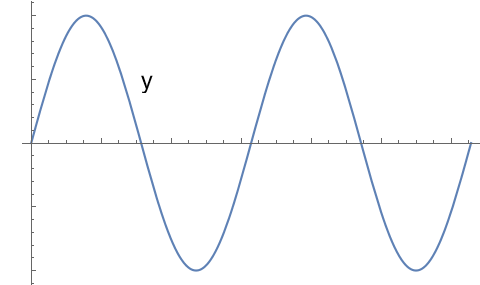
\includegraphics[scale=0.8]{Imagenes/Plot_Onda_02.png}
    \caption{Elongación de una onda.}
\end{figure}
\item Amplitud (A): es la distancia entre la elongación máxima y su posición de equilibrio.
\begin{figure}[H]
    \centering
    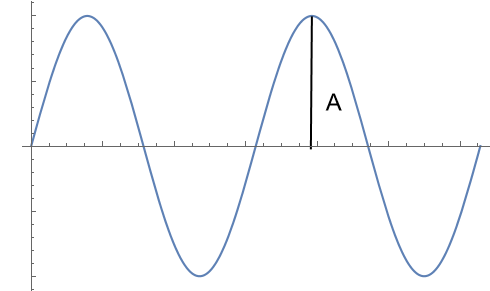
\includegraphics[scale=0.8]{Imagenes/Plot_Onda_03.png}
    \caption{Amplitud de una onda.}
\end{figure}
\item Cresta: cada uno de los puntos más altos de la onda.
\begin{figure}[H]
    \centering
    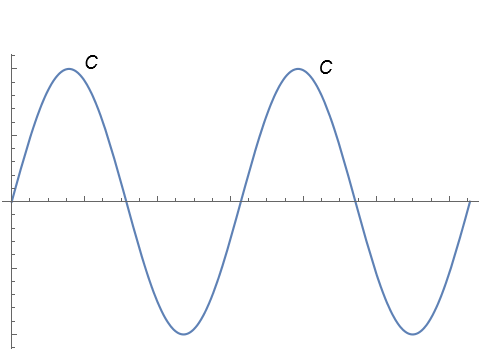
\includegraphics[scale=0.8]{Imagenes/Plot_Onda_04.png}
    \caption{Cresta de una onda.}
\end{figure}
\item Valle: cada uno de los puntos más bajos de la onda.
\begin{figure}[H]
    \centering
    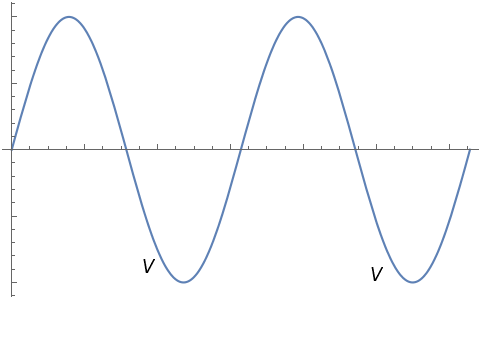
\includegraphics[scale=0.8]{Imagenes/Plot_Onda_05.png}
    \caption{Valle de una onda.}
\end{figure}
\item Ciclo u oscilación: es el recorrido de la onda desde un punto hasta el siguiente punto equivalente.
\begin{figure}[H]
    \centering
    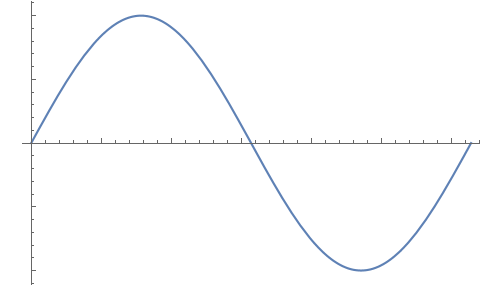
\includegraphics[scale=0.8]{Imagenes/Plot_Onda_06.png}
    \caption{Ciclo u oscilación.}
\end{figure}
\begin{figure}[H]
    \centering
    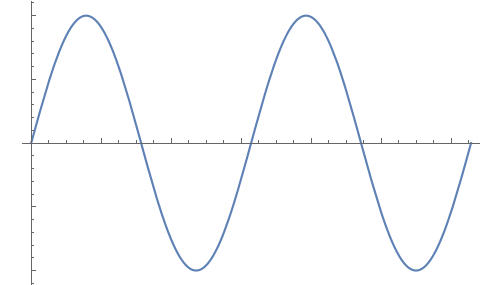
\includegraphics[scale=0.8]{Imagenes/Plot_Onda_06b.png}
    \caption{Ciclo u oscilación.}
\end{figure}
\begin{figure}[H]
    \centering
    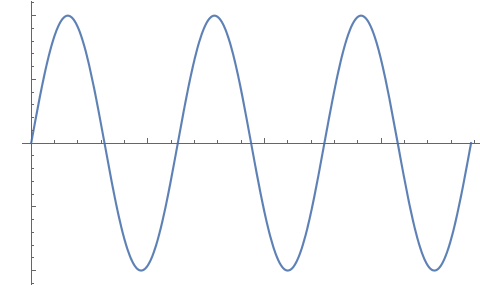
\includegraphics[scale=0.8]{Imagenes/Plot_Onda_06c.png}
    \caption{Ciclo u oscilación.}
\end{figure}
\item Longitud de onda ($\lambda$): es la distancia que separa dos puntos equivalentes consecutivos de la onda.
\begin{figure}[H]
    \centering
    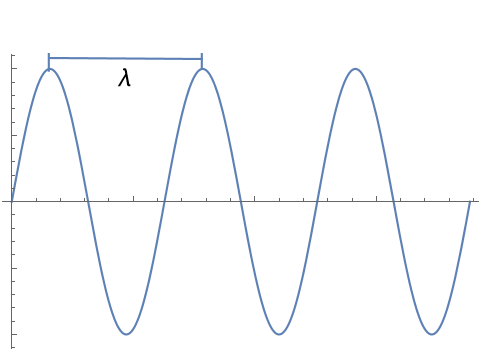
\includegraphics[scale=0.8]{Imagenes/Plot_Onda_07.png}
    \caption{Longitud de onda.}
\end{figure}
\item Periodo (T): es el tiempo que se necesita para hacer una oscilación completa.
\item Frecuencia (f): es el número de oscilaciones o vibraciones que realiza la onda por unidad de tiempo.

El periodo y la frecuencia se relacionan mediante la expresión:
\begin{align*}
f = \dfrac{1}{T}
\end{align*}
\item Frecuencia angular ($\omega$): es la velocidad a la que la onda realiza las oscilaciones.
\begin{eqnarray*}
\begin{aligned}
\omega = \dfrac{2 \cdot \pi}{T} =  2 \cdot \pi \cdot f
\end{aligned}
\end{eqnarray*}
\item Velocidad de propagación (v): es la velocidad a la que se propaga la onda.
\begin{eqnarray*}
\begin{aligned}
v = \dfrac{\lambda}{T} =  \lambda \cdot f
\end{aligned}
\end{eqnarray*}
\end{enumerate}


\section{Expresión para una onda.}

\subsection{Fórmula matemática}

Toda onda requiere de una expresión general que recupera las propiedades mencionadas previamente. La función matemática que nos permite describir el movimiento de una onda siempre es de la siguiente forma:
\begin{align*}
y = f (x \pm v \cdot t)
\end{align*}
Donde:
\begin{enumerate}
\item $y$ es la elongación de la onda.
\item $x$ es la distancia desde el punto estudiado hasta el origen de la onda.
\item $v$ es la velocidad de propagación de la onda.
\item $t$ es el instante de tiempo.
\item El signo delante de la velocidad de propagación indica si la onda mecánica se desplaza hacia la derecha (signo negativo) o hacia la izquierda (signo positivo).
\end{enumerate}


\subsection{Ejercicios.}

Con la finalidad de repasar los conceptos y a la vez, plantear una estrategia para resolver ejercicios, que se recomienda ampliamente para que se ocupe en cada ejercicio.

Se presenta la siguiente estrategia de solución:
\begin{enumerate}
\item Datos.
\item Expresión(es)
\item Sustitución.
\item Resultado (con unidades)
\end{enumerate}
    
\textbf{Enunciado del Ejercicio 1: } Un péndulo de un metro de longitud oscila con un período de \SI{0.31944}{\second}. ¿Cuál es su frecuencia? ¿Cuántas oscilaciones dará en medio minuto?

Datos:  Periodo \, $T = \SI{0.31944}{\second}$

Expresión(es):
\begin{eqnarray*}
\begin{aligned}
f &= \dfrac{1}{T} \\[0.5em] 
f &= \dfrac{\text{oscilaciones}}{\text{tiempo}}  \hspace{0.5cm} \Rightarrow \hspace{0.5cm} \text{oscilaciones} = f \cdot \text{tiempo}
\end{aligned}
\end{eqnarray*}

Sustitución:
\begin{eqnarray*}
\begin{aligned}
f &= \dfrac{1}{T} =  \dfrac{1}{\SI{0.31944}{\second}} =  \SI{3.1304}{\hertz} \\[0.5em] 
\text{oscilaciones} &= f \cdot \text{tiempo} = \\[0.5em] 
&= (\SI{3.1304}{\hertz})(\SI{30}{\second}) = \\[0.5em]  
&= 93.91 \, \text{oscilaciones}
\end{aligned}
\end{eqnarray*}

\textbf{Enunciado del ejercicio 2: } La frecuencia cardiaca de una persona que está desarrollando una actividad física es de 120 latidos por minuto: ¿Cúal es su período de oscilación? Si la actividad física duró \SI{35}{\minute}, ¿cuántos latidos dio el corazón?

Datos:
\begin{eqnarray*}
\begin{aligned}
120 \, \text{lpm}  \hspace{0.3cm} &\Rightarrow \hspace{0.3cm} \dfrac{120 \, \text{lpm}}{\SI{60}{\second}}  \hspace{0.3cm} \Rightarrow \hspace{0.3cm} f = \SI{2}{\hertz} \\[0.5em] 
t &= \SI{35}{\minute} =  \SI{2100}{\second}
\end{aligned}
\end{eqnarray*}

Expresiones:
\begin{eqnarray*}
\begin{aligned}
f &= \dfrac{1}{T} =  \hspace{0.5cm} T = \dfrac{1}{f} \\[0.5em] 
\text{oscilaciones} &= f \cdot t 
\end{aligned}
\end{eqnarray*}

Sustitución:
\begin{eqnarray*}
\begin{aligned}
T &= \dfrac{1}{\SI{2}{\hertz}} =  \SI{0.5}{\second} \\[0.5em] 
\text{oscilaciones} &= (\SI{2}{\hertz})(\SI{2100}{\second}) = \\[0.5em] 
&= \num{4.2d3} \, \text{oscilaciones}
\end{aligned}
\end{eqnarray*}

\textbf{Enunciado del ejercicio 3: } En un estanque de agua se produce una onda cuya longitud de onda es $\lambda = \SI{17}{\milli\meter}$ y un período de $T = \SI{0.8}{\second}$ ¿Cúal será la velocidad de la onda? ¿Qué tiempo le tomará recorrer \SI{2}{\meter}?

Datos:
\begin{eqnarray*}
\begin{aligned}
\lambda &= \SI{17}{\milli\meter} =  \SI{17d-3}{\meter}\\[0.5em] 
T &= \SI{0.8}{\second} \\[0.5em] 
d &= \SI{2}{\meter}
\end{aligned}
\end{eqnarray*}

Expresiones:
\begin{eqnarray*}
\begin{aligned}
f &= \dfrac{1}{T} \\[0.5em] 
v &= \lambda \cdot f \\[0.5em] 
v &= \dfrac{d}{t} \hspace{0.5cm} \Rightarrow \hspace{0.5cm} t = \dfrac{d}{v}
\end{aligned}
\end{eqnarray*}

Sustitución:
\begin{eqnarray*}
\begin{aligned}
f &= \dfrac{1}{T} = \dfrac{1}{\SI{0.8}{\second}} =  \SI{1.25}{\hertz} \\[0.5em] 
v &= \lambda \cdot f =  (\SI{17d-3}{\meter})(\SI{1.25}{\hertz}) = \\[0.5em] 
&= \SI[per-mode=fraction]{0.02125}{\meter\per\second} =  \SI[per-mode=fraction]{2.125d-2}{\meter\per\second} \\[0.5em] 
t &= \dfrac{d}{v} =  \dfrac{\SI{2}{\meter}}{\SI[per-mode=fraction]{2.125d-2}{\meter\per\second}} =  \SI{94.117}{\second}
\end{aligned}
\end{eqnarray*}

\textbf{Enunciado del ejercicio 4: } En un tanque de agua, la orilla del mismo se encuentra a una distancia de \SI{80}{\centi\meter} del punto donde una piedra cayó, se registra que el tiempo entre la caída de la piedra y la llegada de la onda a la orilla siendo de \SI{12}{\second}. Si la onda tiene una longitud de onda es de \SI{14}{\milli\meter}, ¿Qué velocidad tiene la onda? ¿Cuál es la frecuencia de oscilación?


Datos:
\begin{eqnarray*}
\begin{aligned}
d &= \SI{0.8}{\meter} \\[0.5em] 
t &= \SI{12}{\second} \\[0.5em] 
\lambda &= \SI{14}{\milli\meter}
\end{aligned}
\end{eqnarray*}

Expresiones:
\begin{eqnarray*}
\begin{aligned}
v &= \dfrac{d}{t} \\[0.5em] 
f &= \dfrac{v}{\lambda}
\end{aligned}
\end{eqnarray*}

Sustitución:
\begin{eqnarray*}
\begin{aligned}
v &= \dfrac{d}{t} =  \dfrac{\SI{0.8}{\meter}}{\SI{12}{\second}} =  \SI[per-mode=fraction]{6.66667d-2}{\meter\per\second} \\[1em] 
f &= \dfrac{v}{\lambda} =  \dfrac{\SI[per-mode=fraction]{6.66667d-2}{\meter\per\second}}{\SI{14d-3}{\meter}} = \\[0.5em] 
&= \SI{4.7619}{\hertz}
\end{aligned}
\end{eqnarray*}


\section{Tipos de ondas.}

\subsection{Dirección de las ondas.}

De acuerdo con la dirección en la que una onda hace vibrar a las partículas del medio material,  los movimientos ondulatorios se clasifican en: longitudinales y transversales.

\subsection{Ondas longitudinales.}

Las ondas longitudinales se presentan cuando las partículas del medio material vibran paralelamente a la dirección de propagación de la onda.
\begin{figure}[H]
    \centering
    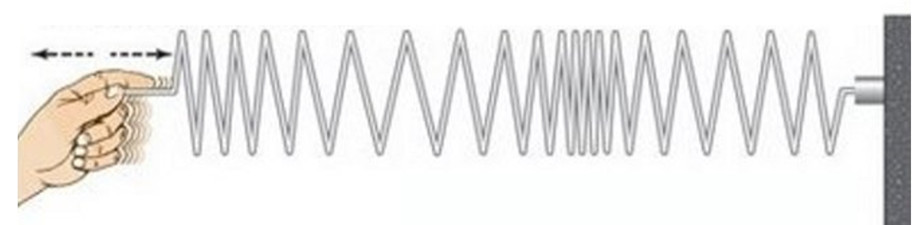
\includegraphics[scale=0.35]{Imagenes/Ondas_07.jpg}
    \caption{Onda longitudinal.}
\end{figure}

Ahora revisaremos un par de propiedades importantes de las ondas longitudinales, la compresión y la rarefacción.

\begin{figure}[H]
    \centering
    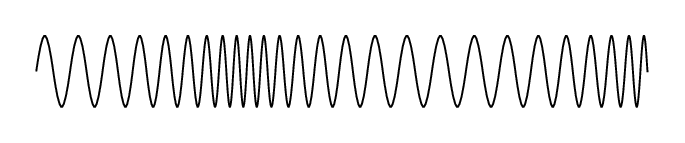
\includegraphics[scale=0.5]{Imagenes/Reflexion_Ondas_05.png}
    \caption{Un tren de ondas viajando de manera horizontal.}
\end{figure}

De la figura anterior, reconocemos dos regiones de interés en la onda:

\begin{enumerate}
\item Compresión.
\item Rarefaccción (expansión).
\end{enumerate}
{
\begin{figure}[H]
    \centering
    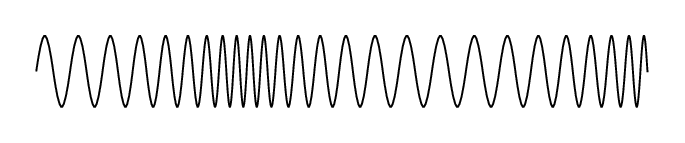
\includegraphics[scale=0.7]{Imagenes/Reflexion_Ondas_05.png}
    \caption{Reflexión de una onda.}
\end{figure}
\begin{tikzpicture}[overlay]
    \draw [line width=0.1cm, color=lavenderindigo] (1.5, 4.5) -- (4.8, 4.5) node [above, midway] {Rarefacción};
    \draw [line width=0.1cm, color=lava] (5.2, 4.5) -- (6.8, 4.5) node [above, midway] {Compresión};
\end{tikzpicture}
}
Las regiones densas en las que gran número de moléculas se agrupan acercándose mucho entre sí se llaman compresiones. Una compresión corresponde a una región de alta presión. Las regiones que tienen relativamente pocas moléculas se conocen como rarefacciones y corresponden a zonas de baja presión.

Las compresiones y rarefacciones se alternan a través del medio en la misma forma que las partículas de aire individuales oscilan de un lado a otro en la dirección de la propagación de la onda.
    
% Tal es el caso de las ondas producidas en un resorte,
% como el de la figura 10.1, el cual se comporta como un oscilador
% armónico cuando se tira del cuerpo suspendido en
% su parte inferior y comienza a oscilar de abajo hacia arriba,
% produciendo ondas longitudinales.
% 

\subsection{Ondas transversales.}

Se presentan cuando las partículas del medio material vibran perpendicularmente a la dirección de propagación de la onda.
\begin{figure}[H]
    \centering
    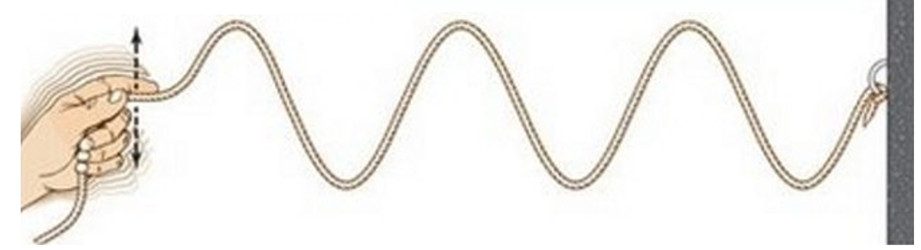
\includegraphics[scale=0.35]{Imagenes/Ondas_08.jpg}
    \caption{Onda transversal.}
\end{figure}

Éstas se producen, por ejemplo, cuando se arroja una piedra en un estanque; al entrar en el agua, expulsa el líquido en todas direcciones; por tanto, unas moléculas empujan a otras, formándose prominencias y depresiones circulares alrededor de la piedra.
\begin{figure}[H]
    \centering
    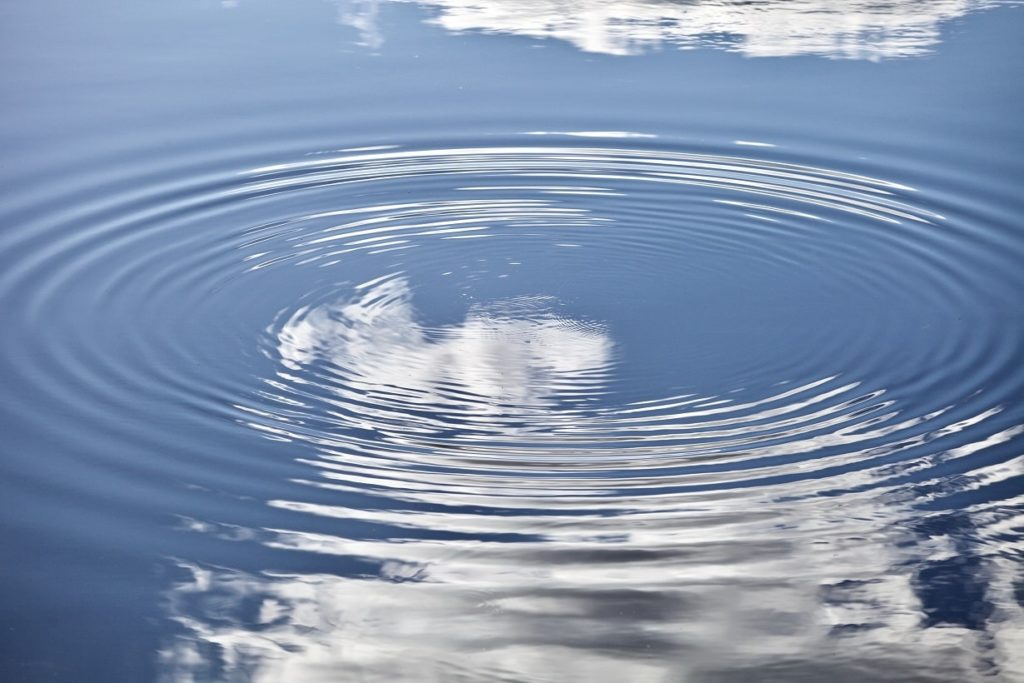
\includegraphics[scale=0.25]{Imagenes/Ondas_06.jpg}
    \caption{Otra onda transversal}
\end{figure}

Como las moléculas de agua vibran (oscilan), hacia arriba y hacia abajo, en forma perpendicular a la dirección en la que se propaga la onda, ésta recibe el nombre de transversal.

\subsection{Energía y ondas.}

En las ondas mecánicas la que se desplaza o avanza es la energía de la onda y no las partículas del medio, pues éstas únicamente vibran u oscilan transmitiendo la energía, pero conservan sus posiciones alrededor de puntos más o menos fijos.

En general, las ondas mecánicas transmiten la energía por medio de la materia, debido a las perturbaciones ocasionadas en ella, pero sin que implique un desplazamiento total de la materia.

\section{Ondas en movimiento.}

\subsection{Reflexión.}

La reflexión de las ondas se presenta cuando éstas encuentran un obstáculo que les impide propagarse,  chocan y cambian de sentido sin modificar sus demás características.

En las siguientes figuras vemos cómo se refleja una onda lineal en donde uno de los extremos está fijo.
\begin{figure}[H]
    \centering
    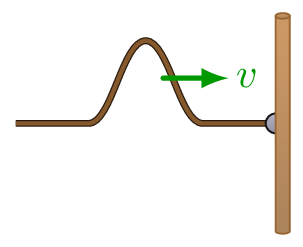
\includegraphics[scale=0.7]{Imagenes/Reflexion_Ondas_01.png}
    \caption{Onda llegando a una superficie.}
\end{figure}
\begin{figure}[H]
    \centering
    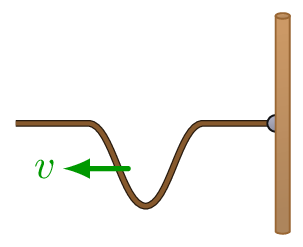
\includegraphics[scale=0.7]{Imagenes/Reflexion_Ondas_02.png}
    \caption{Onda reflejada.}
\end{figure}

En las siguientes figuras veremos cómo se presenta la reflexión de una onda, donde uno de los extremos no está fijo.
\begin{figure}[H]
    \centering
    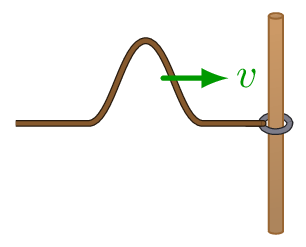
\includegraphics[scale=0.7]{Imagenes/Reflexion_Ondas_03.png}
    \caption{Cuerda con un extremo no fijo.}
\end{figure}
\begin{figure}[H]
    \centering
    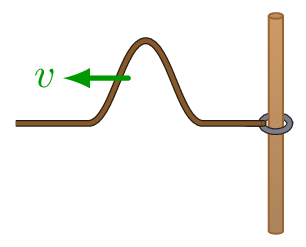
\includegraphics[scale=0.7]{Imagenes/Reflexion_Ondas_04.png}
    \caption{La onda reflejada, mantiene la misma orientación y viaja en la dirección opuesta.}
\end{figure}

% % Una onda producida en un estanque también se refleja al chocar.
% %  El ángulo de reflexión de la onda es igual al ángulo
% % de choque.
% % 

\section{Superposición.}

\subsection{Tren de ondas.}

Si a una cuerda tensa y sujeta por uno de sus extremos se le da un impulso moviéndola hacia arriba, se produce una onda que avanza por las partículas de la cuerda. Éstas ondas se moverán al llegarles el impulso y recobrarán su posición de reposo cuando la onda pase por ellas.

Si la cuerda se sigue moviendo hacia arriba y hacia abajo, producirá un tren de ondas periódico si el movimiento también es periódico.
\begin{figure}[H]
    \centering
    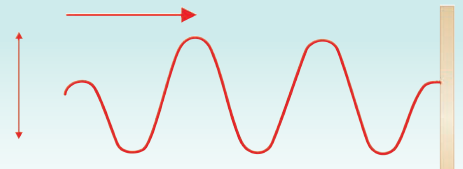
\includegraphics[scale=0.8]{Imagenes/Tren_Onda_01.png}
    \caption{Un tren de ondas.}
\end{figure}
Al dejar caer una piedra en un estanque, como ya mencionamos, se forman ondas transversales.
\begin{figure}[H]
    \centering
    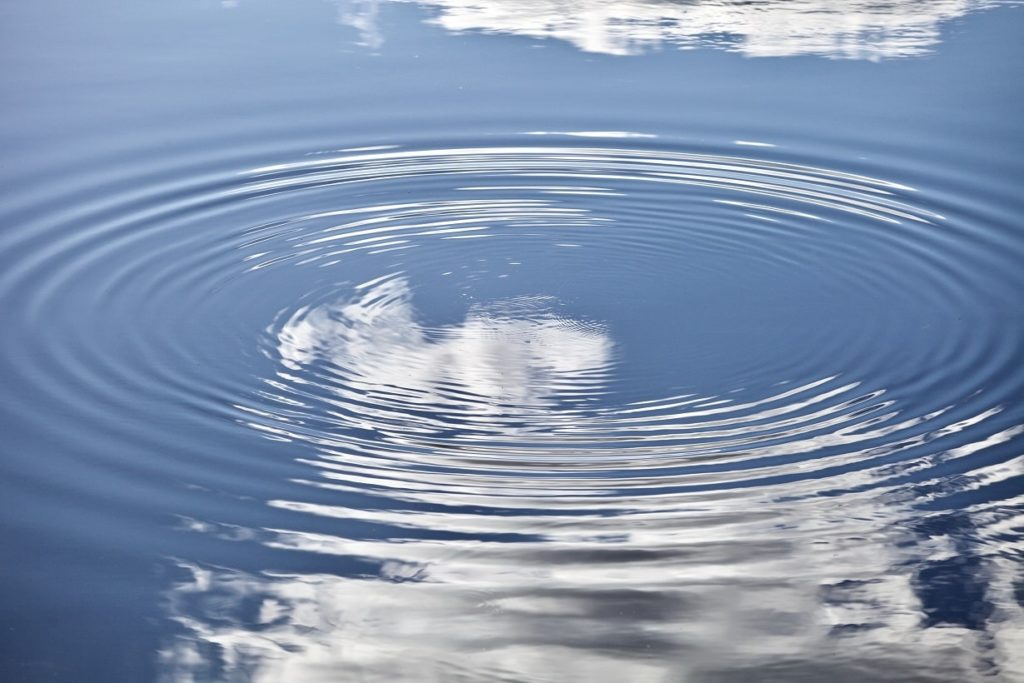
\includegraphics[scale=0.25]{Imagenes/Ondas_06.jpg}
    \caption{Ondas en un estanque.}
\end{figure}
Si los círculos de la imagen anterior representan todos los puntos de una onda que experimentan la misma fase, ya sea una cresta o un valle, al propagarse la onda los círculos se desplazarán generando otros de mayor tamaño. 

Cada círculo representa un frente de onda formado por todos los puntos de la onda con la misma fase,  por eso puede decirse que cada punto de un frente de onda es un nuevo generador de ondas. A partir del centro emisor de las ondas, es decir, del lugar donde cayó la piedra, los diferentes frentes de una onda avanzan al mismo tiempo y con una magnitud de velocidad constante.

Un rayo o vector de propagación es la línea que señala la dirección en que avanza cualquiera de los puntos de un frente de onda. Cuando el medio en que se propaga la onda es homogéneo, la dirección de los rayos siempre es perpendicular o normal al frente de onda.
\begin{figure}[H]
    \centering
    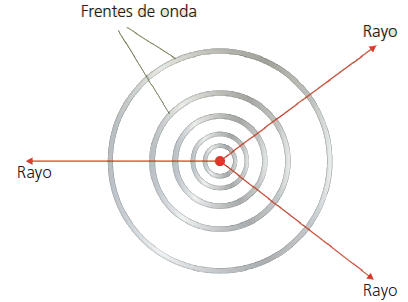
\includegraphics[scale=0.8]{Imagenes/Frente_Onda_01.png}
    \caption{Rayo o vector de propagación.}
\end{figure}

\subsection{Principio de superposición.}

Experimentalmente se ha comprobado que al producirse dos o más trenes de onda al mismo tiempo, en medios elásticos que conservan una proporcionalidad entre la deformación y la fuerza restauradora, cada onda se propaga en forma independiente. Por tanto, la superposición es el desplazamiento que experimenta una partícula vibrante, equivalente a la suma vectorial de los desplazamientos que cada onda le produce.

Una aplicación útil de este principio se presenta cuando desea estudiarse un movimiento ondulatorio formado por muchos trenes de onda para lo cual se descompone en cada uno de sus trenes constituyentes.
\begin{figure}[H]
    \centering
    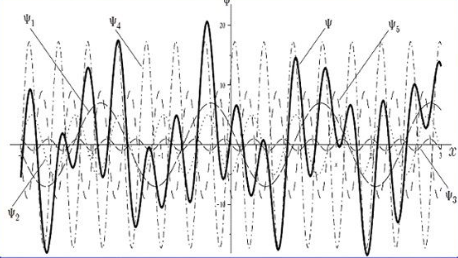
\includegraphics[scale=0.7]{Imagenes/Tren_Onda_02.png}
    \caption{Análisis de tren de ondas.}
\end{figure}

\section{Interferencia de ondas.}

\subsection{Definición.}

La interferencia se produce cuando se superponen simultáneamente dos o más trenes de onda; este fenómeno se emplea para comprobar si un movimiento es ondulatorio o no.

\subsection{Interferencia constructiva.}

La interferencia constructiva se presenta al superponerse dos movimientos ondulatorios de la misma frecuencia y longitud de onda, que llevan el mismo sentido.

Las dos ondas superpuestas se representan por medio de líneas punteadas en la siguiente figura:
\begin{figure}[H]
    \centering
    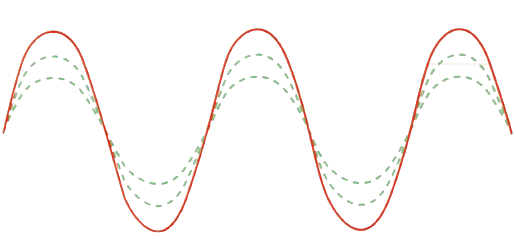
\includegraphics[scale=0.8]{Imagenes/Onda_Constructiva.png}
    \caption{Interferencia constructiva.}
\end{figure}


\subsection{Interferencia destructiva.}

La interferencia destructiva se presenta cuando se superponen dos movimientos ondulatorios con una diferencia de fase. Por ejemplo, al superponerse una cresta y un valle de diferente amplitud con una diferencia de fase igual a media longitud de onda, la onda resultante tendrá menor amplitud.
\begin{figure}[H]
    \centering
    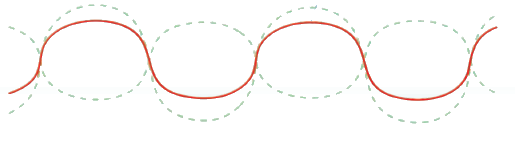
\includegraphics[scale=0.8]{Imagenes/Interferencia_Desctructiva_02.png}
    \caption{La línea sólida es la onda resultante con su amplitud menor a las ondas que presentan interferencia.}
\end{figure}
Pero si se superponen dos ondas de la misma amplitud con una diferencia de fase equivalente a media longitud de onda, es decir $\ang{180}$, la suma vectorial de sus amplitudes contrarias será igual a cero, por consiguiente, la onda resultante tendrá una amplitud nula.
\begin{figure}[H]
    \centering
    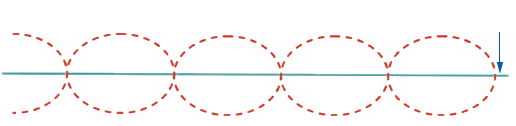
\includegraphics[scale=0.8]{Imagenes/Interferencia_Desctructiva_03.png}
    \caption{Cuando las ondas tienen una fase de \ang{180}, se cancelan al interactuar, obteniendo una línea plana, es decir, no hay una onda resultante como tal.}
\end{figure}

% \section{Ondas estacionarias.}

% \subsection{Definición.}

% Las ondas estacionarias se producen cuando interfieren dos movimientos ondulatorios de la misma frecuencia y amplitud que se propagan en diferente sentido a lo largo de una línea con una diferencia de fase de media longitud de onda.

\section{Refracción de ondas.}

\subsection{Definición de la refracción.}

La refracción de ondas se presenta cuando éstas pasan de un medio a otro de distinta densidad. También cuando el medio es el mismo, pero se encuentra en condiciones diferentes, por ejemplo, el agua a distintas profundidades. Ello origina que las ondas cambien su magnitud de velocidad de propagación y su longitud de onda, conservando constante su frecuencia.

Consideremos que un tren de ondas periódico cruza la zona entre dos medios de distinta densidad.
\begin{figure}[H]
    \centering
    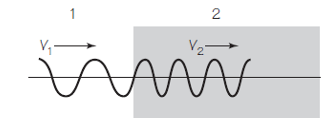
\includegraphics[scale=1]{Imagenes/Refraccion_Ondas_02.png}
    \caption{Tren de ondas interactuando en dos medios con distinta densidad.}
\end{figure}

Suposición para la refracción de ondas:
\begin{enumerate}
\item La velocidad de la propagación en el medio 1 es mayor que en el medio 2.
\item Para simplificar suponemos que toda la onda se transmite y nada se refleja.
\item El patrón de onda periódico también se comprime.
\end{enumerate}
Por lo tanto, la longitud de onda $\lambda_{2}$ de la onda transmitida es más corta que la longitud de onda $\lambda_{1}$ de la onda entrante o incidente.
\begin{figure}[H]
    \centering
    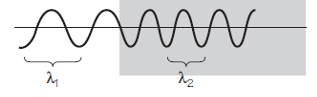
\includegraphics[scale=1]{Imagenes/Refraccion_Ondas_03.png}
    \caption{Longitud de onda $\lambda_{2}$ en el medio 2.}
\end{figure}
Aunque la longitud de onda cambia cuando la onda pasa a través del límite, la frecuencia de la onda no puede cambiar.

Si el medio es continuo (una cuerda que no está rota), ambos lados del límite deben subir y bajar juntos. Las frecuencias de las ondas incidentes y transmitidas deben, entonces, ser iguales, podemos simplemente etiquetar ambas como $f$.

La relación entre longitud de onda, frecuencia y velocidad para las ondas incidentes y transmitidas se puede escribir por separado como:
\begin{align*}
\lambda_{1} \, f &= v_{1} \\[0.5em]
\lambda_{2} \, f &= v_{2}
\end{align*}
Dividiendo una ecuación por la otra, eliminado $f$, obtenemos que:
\begin{align*}
\dfrac{\lambda_1}{\lambda_{2}} = \dfrac{v_{1}}{v_{2}}
\end{align*}
La ecuación anterior nos dice que la razón entre las longitudes de onda en dos medios es igual a la razón entre las velocidades de propagación de las ondas en esos medios.


\section{Difracción de ondas.}

\subsection{Definición de la difracción.}

Cuando una onda encuentra un obstáculo en su camino y lo rodea o sigue su contorno  se produce la difracción de ondas.
\begin{figure}[H]
    \centering
    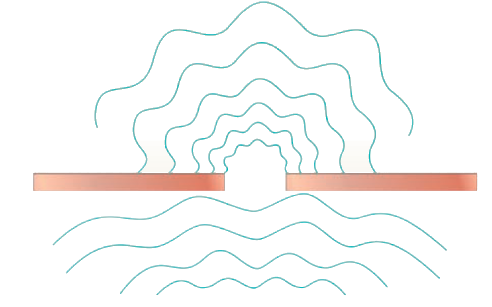
\includegraphics[scale=0.6]{Imagenes/Difraccion_01.PNG}
\end{figure}
Este fenómeno es más notorio a medida que son mayores las longitudes de onda, y si el tamaño de la abertura por la que atravesará la onda es menor.
\begin{figure}[H]
    \centering
    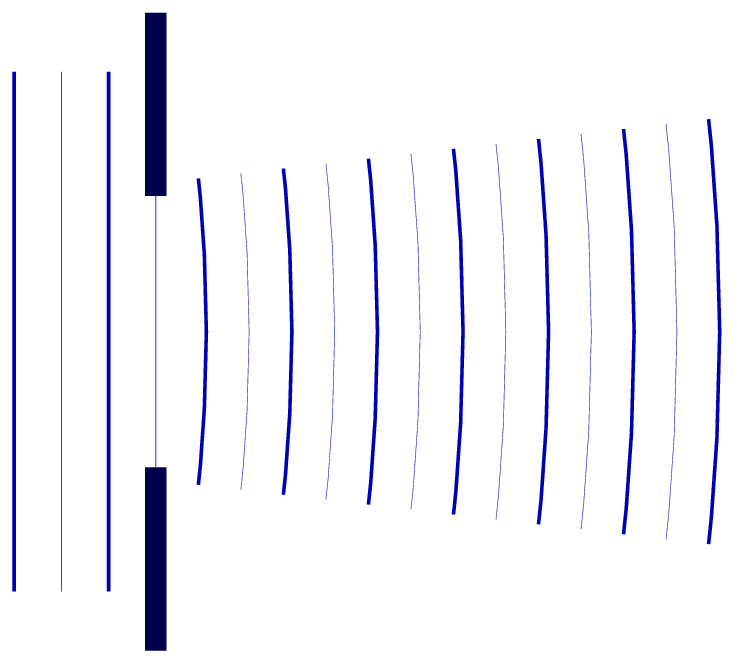
\includegraphics[scale=0.25]{Imagenes/Difraccion_Patrones_01.png}
    \caption{Grandes aberturas - Poca difracción.}
\end{figure}
En la siguiente figura se aprecia otro caso de la difracción de ondas.
\begin{figure}[H]
    \centering
    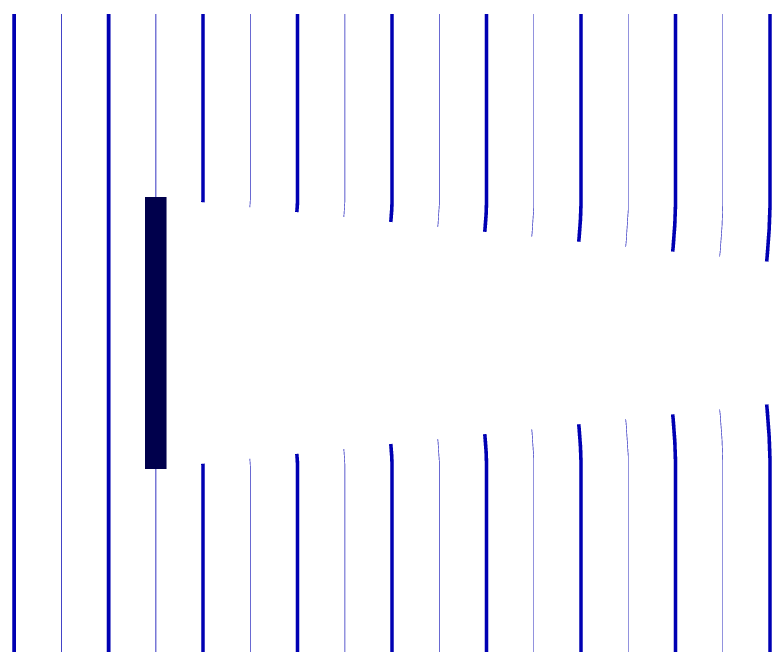
\includegraphics[scale=0.25]{Imagenes/Difraccion_Patrones_02.png}
    \caption{No hay abertura - la onda rodea al obstáculo.}
\end{figure}
En la siguiente figura se muestra el caso de cuando se tiene una pequeña abertura y el resultado en la difracción de la onda.
\begin{figure}[H]
    \centering
    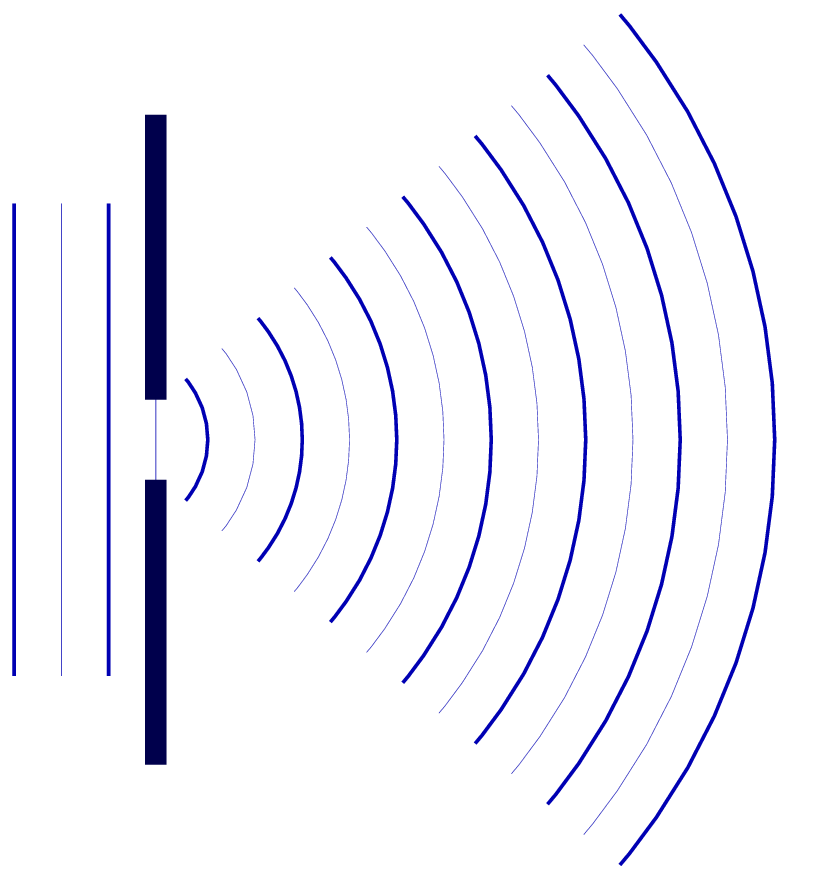
\includegraphics[scale=0.15]{Imagenes/Difraccion_Patrones_03.png}
    \caption{Pequeñas aberturas - Mucha difracción.}
\end{figure}



\end{document}